Se utilizan para la comunicación inalámbrica como la radio, televisión, teléfonos móviles, Wi-Fi, antenas y satélites. Abarca frecuencias desde 30 Hz hasta 300 GHz.

\subsection{Señales AM y FM}

Las ondas de radio se transmiten mediante señales AM y FM.

\textbf{AM}, o \textbf{amplitud modulada}, cambia la amplitud de la señal. Viajan una mayor distancia y son más simples de recibir. Son más susceptibles a interferencias y ruido, lo que resulta en una peor calidad.

\textbf{FM}, o \textbf{frecuencia modulada}, cambia la frecuencia de la señal. Viajan una menor distancia y son más complejas de recibir. Son menos susceptibles a interferencias y ruido, lo que resulta en una mejor calidad.

\begin{figure}[H]
  \centering
  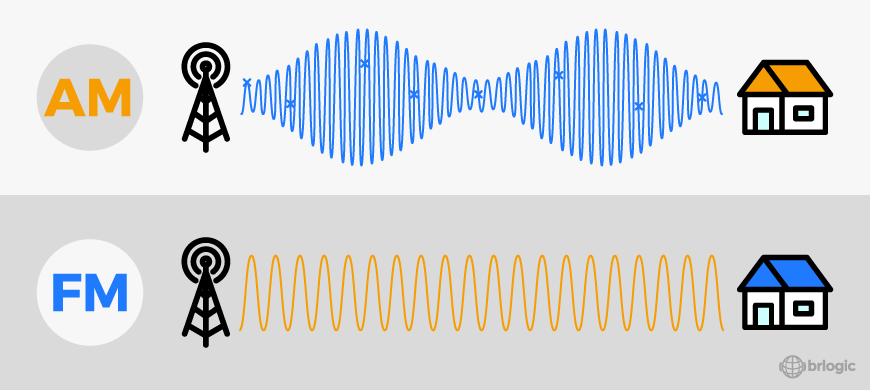
\includegraphics[scale=0.4]{imagenes/am_fm.png}
  \caption{Señales AM y FM\cite{brlogicamfm}}
\end{figure}

\subsection{Propagación en la Ionósfera}

La \textbf{ionósfera}, una capa electricamente cargada de la atmósfera, es crucial en la propagación de ondas de radio. Se ubica aproximadamente entre los 60 y 1000 km de altura sobre la superficie terrestre. Contiene gases ionizados que pueden reflejar, refractar y absorber las ondas de radio, permitiendo así la comunicación a larga distancia. Para enviar ondas se usa un transmisor y para recibirlas un receptor.

\begin{figure}[H]
  \centering
  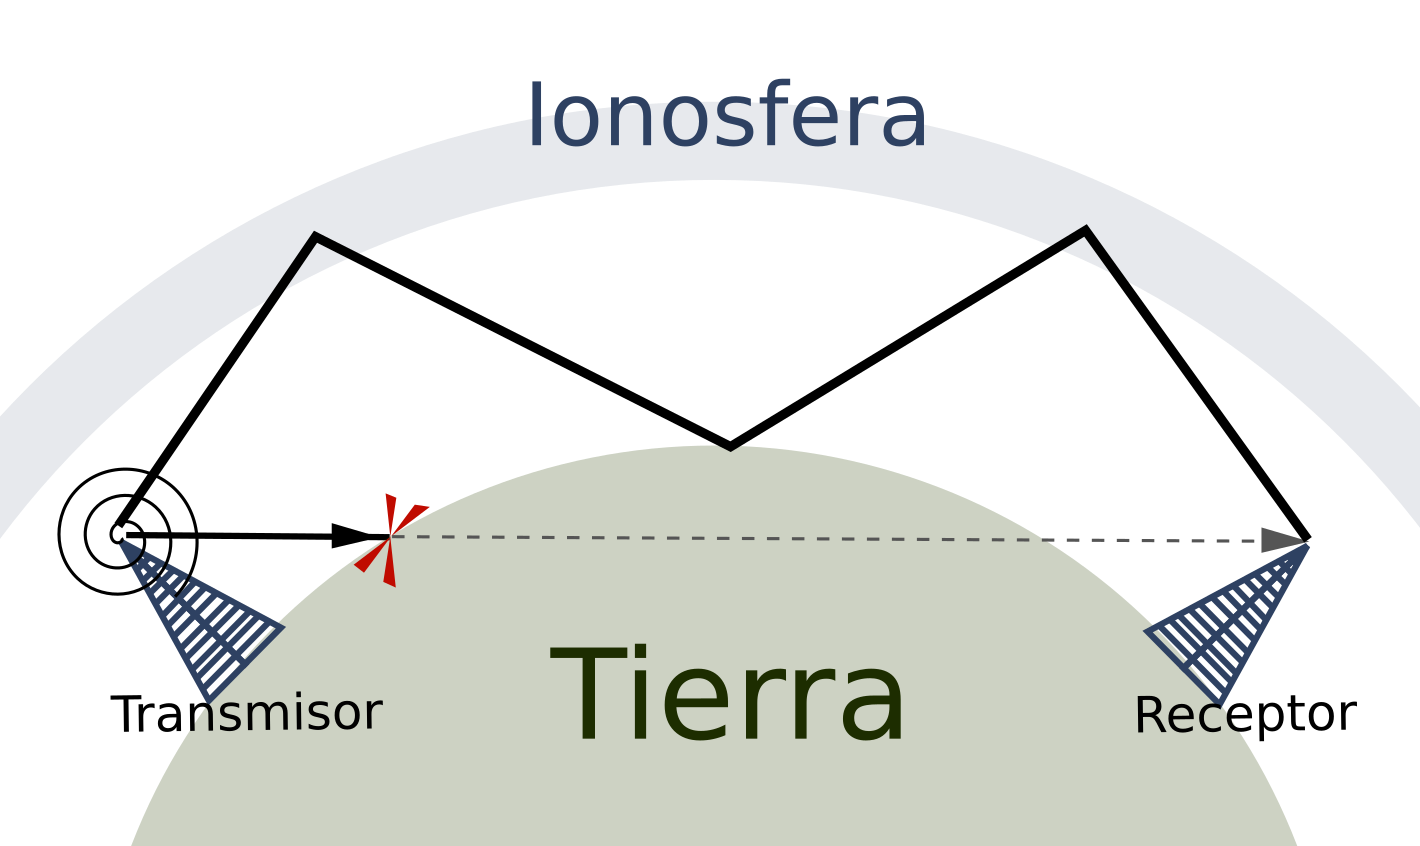
\includegraphics[scale=0.8]{imagenes/ionosfera_onda.png}
  \caption{Ondas reflejadas en la ionósfera\cite{wikiionosfera}}
\end{figure}
